\documentclass[10pt,conference,compsocconf]{IEEEtran}

\usepackage{hyperref}
\usepackage{graphicx}	% For figure environment


\begin{document}
\title{Machine Learning Course - Project 1}

\author{
  Victor Faramond, Mathieu Schopfer, Dario Anongba Varela\\
  \textit{Department of Computer Science, EPFL Lausanne, Switzerland}
}

\maketitle

\section{Introduction}

This report concerns project 1 of PCML. This project consisted in using machine learning algorithms on datasets provided by the CERN. The aim was to classify events measured by the ATLAS experiment to distinguish events originating in the Higgs boson decay from background.

\section{Models and Methods}

\subsection{Data}

Two sets of data were provided in the form of csv files, a \textit{training} and a \textit{test} set. The input of both sets consists in $D=30$ feature columns $\mathbf{x}_n$. In the training set, an additionnal output column $y_n$ is provided. The output is binary (-1 or 1), depending whether the recorded signal corresponds to an actual event (1) or to background noise (-1).

\subsection{Pre-processing}
\subsubsection{Missing data} % Je crois que "missingness" signifie "disparition" (genre d'enfant)
After an exploratory data analysis phase, we found that only a quarter of the dataset is complete. 11 variables out of 30 have missing records which are designated by $-999$. However, we found a clear structure about these missing values. Most of them are related to the \textit{jet} properties. If an event contains no jet at all, all the jet related features are missing. If an event contains only one jet, the leading jet features are present but the subleading jet features are missing. Therefore, in the ridge regression case (see below), we decided to split the dataset into three different subsets corresponding to the jet values $\{0\}$, $\{1\}$ and $\{2, 3\}$, drop the columns with missing values and train a specific classifier on each subset.

\subsubsection{Missing values imputing}
Missing values are first imputed. For a given input column $x_{\bullet,i}$ ($i \in \{1, ..., D\}$) missing values are replaced in both the training and the test sets by the value appearing most frequently in column $x_{\bullet,i}$ of the training set.

\subsubsection{Feature engineering}
For all the positive value columns, we added a corresponding column with the inverse log values of the column,

\[
x_{\bullet,i} \to \frac{1}{1+\log x_{\bullet,i}}.
\]

Thus, we can reduce the range of the values.

\subsubsection{Standardization}
We standardized both the training and test datasets using the mean and the variance of the training set.

\section{Machine learning models}

\subsection{Models}

The following models were tested:
\begin{itemize}
\item Gradient and stochastic gradient descent, $\gamma=0.01$
\item Least squares
\item Ridge regression, with polynom basis, $\lambda=0.6$
\item Logistic and regularized logistic regression, $\gamma=0.6, \lambda=0.04$
\end{itemize}

\subsubsection{Ridge regression}
Before fitting the ridge regression model, we added polynomial features to our training and test sets:

\begin{itemize}
\item The square root $\sqrt{\mathbf{x}_n}$ of the feature.
\item $\mathbf{x}_n^k$, for $k\in \{1, ..., d\}$. The parameter $d$ is different for each subset of data (regarding the number of jets) and has been defined using a grid search with values of $d \in \{1, ..., 11\}$. See figure \ref{jet_0_degress}.
\item The products $x_{\bullet,i}\cdot x_{\bullet,j}$, $\forall i,j \in \{1, ..., D\}$.
\end{itemize}

\begin{figure*}[htp]
\centering
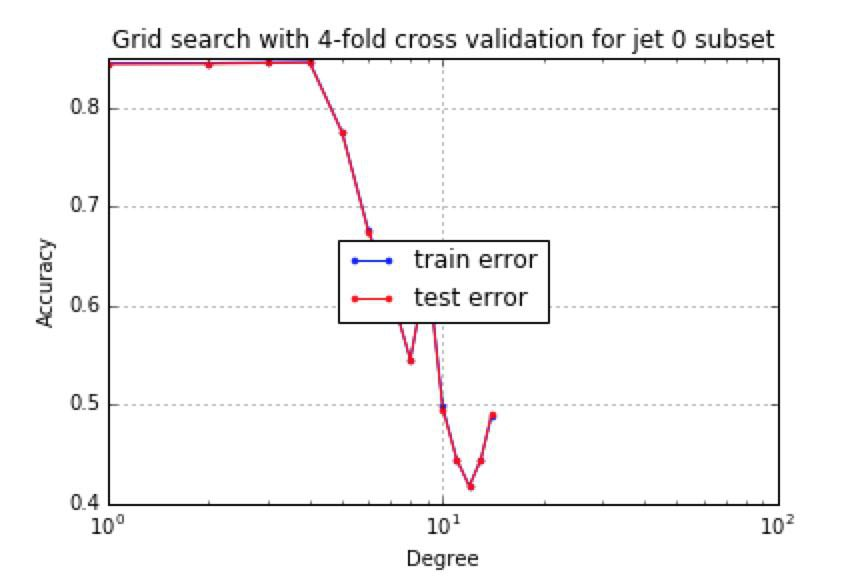
\includegraphics[scale=0.5]{grid_search_jet_0_degrees.png}
\caption{\label{jet_0_degress} Mean accuracy of the ridge regression model on data subset verifying jet=0, for various values of maximal polynomial degree.}
\end{figure*}

The parameter $\lambda$ was also defined using a grid search with values of $\lambda \in {1e-9, ..., 1e+1}$. See figure \ref{jet_0_lambdas}.

\begin{figure*}[htp]
\centering
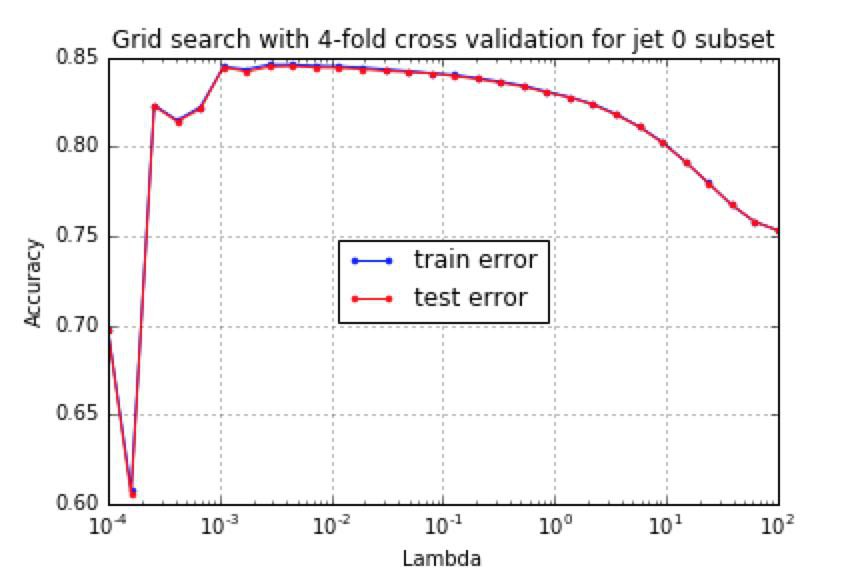
\includegraphics[scale=0.5]{grid_search_jet_0_lambdas.png}
\caption{\label{jet_0_lambdas} Mean accuracy of the ridge regression model on data subset verifying jet=0, for various values of $\lambda$.}
\end{figure*}

\subsection{Cross validation}

To train and test the various models presented hereabove, a 10-fold cross validation method was used. This consists in splitting the training data set into ten subsets of equivalent size. Then 9 subsets are used to train the models, the last one to test it. This proces is repeated for all 10 combinations of training and testing subsets. This allows us to make sure a model is stable and that we did not overfit on the training set.

\subsection{Assessment of models accuracy}

At each step of the 10-fold cross validation, the positives rate was calculated on the test subset. The positive rates is simply given as the number of model ouptuts $y_n$ agreeing with the (known) expected output divided by the total number of events in the subset.

Then the mean and variance of positives rates was calculated and retained as the model accuracy score.

\subsection{Choice of model for submission}

The model that was choosen for submission was that achieving the highest positives rate score.

\section{Results}

Table \ref{res_table} summarizes the results for all models. Regarding these results, the ridge regression model was selected for submission.

\begin{table*}[htp]
\centering
\begin{tabular}[c]{|c|c|c|}
  \hline
  \textbf{Model} & \textbf{Mean accuracy} & \textbf{Variance} \\
  \hline
  Gradient descent & 0.763168 & 0.000006 \\
  \hline
  Stochastic gradient descent & 0.686248 & 0.000562 \\
  \hline
  Least squares & 0.776600 & 0.000007 \\
  \hline
  Rigde regression & 0.833556 & 0.000002 \\
  \hline
  Logistic regression & 0.679196 & 0.000004 \\
  \hline
  Regularized logistic regression & 0.679196 & 0.000004 \\
  
  \hline
\end{tabular}
\caption{\label{res_table} Mean accuracy and standard deviation for all tested models.}
\end{table*}

\end{document}
